\documentclass[final]{beamer}
\mode<presentation>
\usetheme[mat]{HYposter}

% Change colours on line 3 by setting \usetheme[<id>]{HYposter}.
% The different ids are:
%  maa: Faculty of Agriculture and Forestry 
%  hum: Faculty of Arts 
%  kay: Faculty of Behavioural Sciences 
%  bio: Faculty of Biological and Environmental Sciences 
%  oik: Faculty of Law 
%  med: Faculty of Medicine 
%  far: Faculty of Pharmacy 
%  mat: Faculty of Science 
%  val: Faculty of Social Sciences 
%  teo: Faculty of Theology 
%  ell: Faculty of Veterinary Medicine 
%  soc: Swedish School of Social Science 
%  kir: University of Helsinki Library
%  avo: Open University
%  ale: Aleksanteri Institute
%  neu: Neuroscience Institute
%  biot: Bioscience Institute
%  atk: Computer centre
%  rur: Ruralia Institute
%  koe: Laboratory animal centre
%  kol: Collegium for Advanced Studies
%  til: Center for Properties and Facilities
%  pal: Palmenia
%  kie: Language centre
% Without options a black theme without faculty name will be used.

\usepackage[english]{babel}
\usepackage[T1]{fontenc}
\usepackage[utf8]{inputenc}
\usepackage{lmodern}
\usepackage{amsmath,amsthm, amssymb, latexsym}
\usepackage[orientation=portrait,size=a0,scale=1.4]{beamerposter}

% Set up the title and author info
\titlestart{Pretty Posters With \LaTeX}
\titleend{Using the HYposter Style}
\author{Olli Wilkman$^1$}
\institute{$^1$Department of Physics, \url{olli.wilkman@iki.fi}}
\leftcorner{}

\usefonttheme[onlymath]{serif}

\begin{document}
\begin{poster}

\newcolumn

\section{\LaTeX~posters made easier}
The \texttt{HYposter} style enables you to make scientific posters with a University of Helsinki look using  the \texttt{beamerposter} package for \LaTeX. 

The official poster templates for the university are available only for Microsoft PowerPoint and Adobe InDesign, expensive pieces of software which are not easily available. \LaTeX, on the other hand, is free and works on almost all commonly used computer systems. It also has superior capabilities in typesetting mathematical formulas, which makes it popular among scientists.


\section{The look}
The university has two poster styles, that silly one with the gigantic logo and header taking up a third of the page, and the tighter one. This poster style tries to emulate the second one. Though it does not exactly conform to the official poster style of the university, but it tries to do a good enough job. 

The background of the poster is white and the text is black. The block headings are in the faculty colour. The first line of the poster title is in the faculty colour and the rest in neutral grey. In the lower right corner the name of the university is set in neutral grey and the faculty name in the faculty colour.
Some space for things such as logos of cooperating or supporting institutes is provided in the lower left.

The layout of the official poster and this example is three-column, but you can also use two columns.

It is not possible to use the university's official fonts, not least because of the rather strict license they come under. However, the sans-serif font used here is a reasonable replacement.


\section{Using the package}
\texttt{HYposter} is a style definition for \texttt{beamerposter}, which itself is a package that uses the \texttt{beamer} document class to produce posters. This means you need both \texttt{beamer} and \texttt{beamerposter} in order it to work. Most modern \LaTeX~distributions already come with \texttt{beamer}, and installing the rest is not a problem.

Note that due to some radical redesigns, this style is not compatible with any other \texttt{beamerposter} style, that is, if you write a poster using this style, you cannot simply change the style to another one.

See the \texttt{README} and \texttt{INSTALL} files for more details about installation and usage of the package (though they assume a basic knowledge of \LaTeX).




\newcolumn

\section{Versatility}
This is the cool part: the poster supports \emph{all} of the university's different colour themes. It also automatically changes the name of the faculty or department in the lower right corner. Everything happens under the hood, and the user does not need to worry about the appearance of the poster at all, only the contents.

The style supports all of the university's different faculties and special departments which have an official colour scheme.


\section{The colour options}

The colour scheme of the following faculties and departments is supported. This is a comprehensive list of all the official color schemes defined for our university.

\begin{itemize}
\item Faculty of Agriculture and Forestry 
\item Faculty of Arts 
\item Faculty of Behavioural Sciences 
\item Faculty of Biological and Environmental Sciences 
\item Faculty of Law 
\item Faculty of Medicine 
\item Faculty of Pharmacy 
\item Faculty of Science 
\item Faculty of Social Sciences 
\item Faculty of Theology 
\item Faculty of Veterinary Medicine 
\item Swedish School of Social Science
\item Aleksanteri Institute
\item Center for Information Technology
\item Center for Properties and Facilities
\item Helsinki Collegium for Advanced Studies
\item Institute of Biotechnology
\item Laboratory Animal Centre
\item Language Centre
\item Neuroscience Center
\item Open University
\item Palmenia Centre for Continuing Education
\item Ruralia Institute
\item University of Helsinki Library
\item None (plain black and white)
\end{itemize}


\section{Can I help?}
There are things that still don't work quite as well as I'd like. The math fonts don't seem to always scale properly, and I have been so far unable to fix this.

Contributions and comments are always welcome. Contribute on Github or send email to \url{olli.wilkman@iki.fi}.


\newcolumn

\section{Example 1: math}
You can more or less use all the nice math features of \LaTeX~in your poster:

\begin{equation}
	f(x) = \frac{1}{2}\left(\frac{1}{1+x} + 1\right)
\end{equation}

\begin{equation}
	P_3(x) = a_0 + a_1 x + a_2 x^2 + a_3 x^3
\end{equation}

Unfortunately right now there are still some problems with the scaling of the math fonts:

\begin{equation}
	\sum_{n=0}^\infty \frac{1}{2^n} = 2
\end{equation}



\section{Example 2: Images and References}
Including images is simple.  With pdf\LaTeX, you can use images in many common formats, including PNG and JPEG, though in a poster you should strive to use scaleable graphics, for example in PDF format. Due to a limitation of pdf\LaTeX, EPS graphics do not work, but they can be converted to PDF.
	
Using labels to refer to figures and tables also works like it should, as demonstrated by these references to Figure \ref{examplefigure} and Table \ref{tableexample}.

\begin{figure}
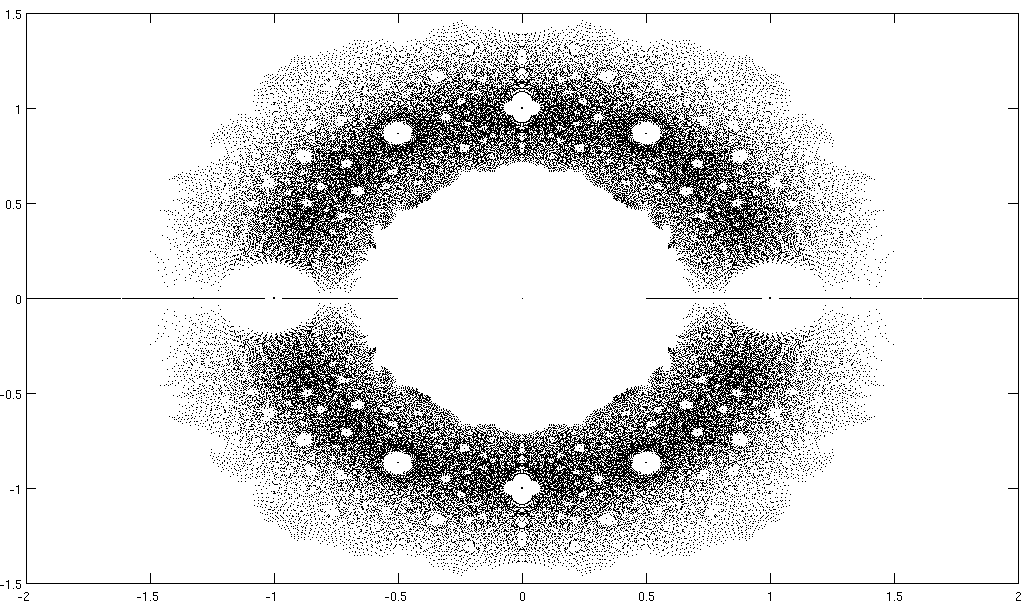
\includegraphics[width=0.8\textwidth]{zeros.png}
\label{examplefigure}
\caption{Some mathematical plot}
\end{figure}

Image courtesy of Janne Korhonen.


\section{Example 3: Tabulated table}

Table environments work, too.

\begin{table}
	\begin{tabular*}{0.5\textwidth}{@{\extracolsep{\fill}} c|r|r|r }
		$x$ & $x^2$ & $x^3$ & $x^4$\\
		\hline
		1 &  1 &   1 &   1 \\
		2 &  4 &   8 &  16 \\
		3 &  9 &  27 &  81 \\
		4 & 16 &  64 & 256 \\
		5 & 25 & 125 & 625 \\
	\end{tabular*}
	\caption{Some natural numbers and their first few powers.\label{tableexample}}
\end{table}

\section{Where can I find it?}
HYposter is hosted at Github for ease of development and cooperation. Get it at \url{https://github.com/dronir/HYposter}.


\end{poster}
\end{document}